\testfile{pgfplotstest.ternarytex}
\testsection{Ternary axes}

\begin{tikzpicture}
%\tracingmacros=2 \tracingcommands=2
	\begin{axis}[axis type=ternary,
%		grid=major,
	]

\def\markpoint(#1);{%
	\node[anchor=base,draw=black,font=\tiny] at (axis cs:#1) {(#1)};
	\filldraw (axis cs:#1) circle(0.5pt);
}

	\addplot3[only marks,scatter,point meta=\coordindex] coordinates {
		(1,0,0)
	%	(0,1,0)
		(0,0,1)
		(1,0,1)
	%	(0,0.5,0.5)
	%	(0.5,0.5,0)
	%	(0.5,0,0.5)
	%	(0.33333,0.33333,0.33333)
	};
	%--------------------------------------------------
	% \draw[red] 
	% 	(axis cs:1,0,0) -- 
	% 	(axis cs:0,1,0) --
	% 	(axis cs:0,0,1) -- cycle;
	%-------------------------------------------------- 

		\markpoint(0.8,0,0.2);
		\markpoint(0.8,0.2,0);
		\markpoint(0,0.8,0.2);

		\markpoint(0.2,0,0.8);
		\markpoint(0.2,0.8,0);
		\markpoint(0,0.2,0.8);
	\end{axis}
\end{tikzpicture}

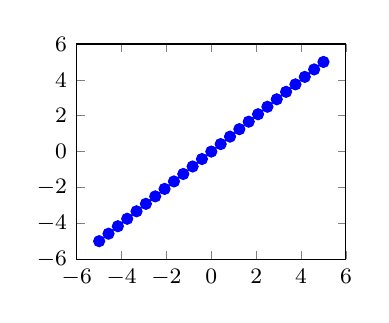
\begin{tikzpicture}
	\begin{axis}[footnotesize]
		\addplot {x};
	\end{axis}
\end{tikzpicture}
